\begin{figure}[H]
\centering
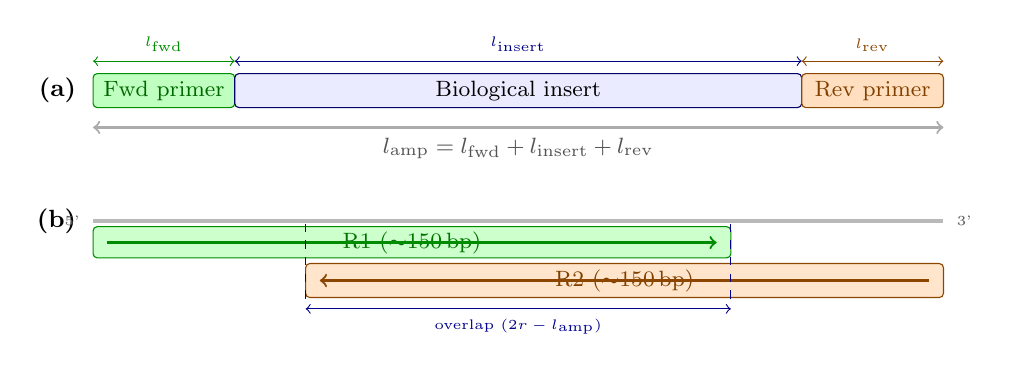
\begin{tikzpicture}[x=0.9cm, y=0.72cm, font=\small]

  % ────────────────────────────────────────────────────────────────────
  % (a)  Amplicon = Fwd primer + Biological insert + Rev primer
  % ────────────────────────────────────────────────────────────────────
  \node[left, font=\small\bfseries] at (-0.1, 0.3) {(a)};

  % Fwd primer block (green, ~2/12 of total)
  \filldraw[fill=green!25, draw=green!55!black, rounded corners=1.5pt]
    (0,0) rectangle (2,0.6);
  \node[font=\footnotesize, green!40!black] at (1,0.3) {Fwd primer};

  % Biological insert block (blue-gray)
  \filldraw[fill=blue!8, draw=blue!40!black, rounded corners=1.5pt]
    (2,0) rectangle (10,0.6);
  \node[font=\footnotesize] at (6,0.3) {Biological insert};

  % Rev primer block (orange, ~2/12 of total)
  \filldraw[fill=orange!25, draw=orange!55!black, rounded corners=1.5pt]
    (10,0) rectangle (12,0.6);
  \node[font=\footnotesize, orange!50!black] at (11,0.3) {Rev primer};

  % Length annotation braces (above)
  \draw[<->, thin, green!55!black]  (0,0.82)  -- (2,0.82)
    node[midway, above, font=\tiny]  {$l_\mathrm{fwd}$};
  \draw[<->, thin, blue!50!black]   (2,0.82)  -- (10,0.82)
    node[midway, above, font=\tiny]  {$l_\mathrm{insert}$};
  \draw[<->, thin, orange!55!black] (10,0.82) -- (12,0.82)
    node[midway, above, font=\tiny]  {$l_\mathrm{rev}$};

  % Amplicon total span (below)
  \draw[<->, thick, gray!65] (0,-0.35) -- (12,-0.35)
    node[midway, below, font=\footnotesize, gray!65!black] {$l_\mathrm{amp} = l_\mathrm{fwd} + l_\mathrm{insert} + l_\mathrm{rev}$};

  % ────────────────────────────────────────────────────────────────────
  % (b)  R1 / R2 read directions and overlap (schematic, ~150 bp reads)
  %      Using proportions: total = 12 u, read length = 9 u → overlap = 6 u
  % ────────────────────────────────────────────────────────────────────
  \node[left, font=\small\bfseries] at (-0.1,-2.0) {(b)};

  % Amplicon backbone
  \draw[very thick, gray!55] (0,-2.0) -- (12,-2.0);
  \node[left,  font=\tiny, gray!70!black] at (-0.05,-2.0) {5'};
  \node[right, font=\tiny, gray!70!black] at (12.05,-2.0) {3'};

  % ── R1: starts at fwd primer, reads rightward, ~150 bp ──
  \filldraw[fill=green!20, draw=green!55!black, rounded corners=1.5pt]
    (0,-2.65) rectangle (9,-2.1);
  \node[font=\footnotesize, green!45!black] at (4.5,-2.38) {R1 ($\sim$150\,bp)};
  \draw[->, thick, green!55!black] (0.2,-2.38) -- (8.8,-2.38);

  % ── R2: starts at rev primer, reads leftward, ~150 bp ──
  \filldraw[fill=orange!20, draw=orange!55!black, rounded corners=1.5pt]
    (3,-3.35) rectangle (12,-2.75);
  \node[font=\footnotesize, orange!50!black] at (7.5,-3.05) {R2 ($\sim$150\,bp)};
  \draw[<-, thick, orange!55!black] (3.2,-3.05) -- (11.8,-3.05);

  % ── Overlap region ──
  \draw[dashed, blue!55!black, thin] (3,-2.05)  -- (3,-3.45);
  \draw[dashed, blue!55!black, thin] (9,-2.05)  -- (9,-3.45);
  \draw[<->, blue!55!black] (3,-3.55) -- (9,-3.55)
    node[midway, below, font=\tiny, blue!55!black]
      {overlap ($2r - l_\mathrm{amp}$)};

\end{tikzpicture}
\caption{(a)~An amplicon consists of the forward primer, the biological insert, and the
reverse primer. The total amplicon length is $l_\mathrm{amp} = l_\mathrm{fwd} +
l_\mathrm{insert} + l_\mathrm{rev}$; BLAST primer localisation reports
$l_\mathrm{amp}$ directly as the span from forward primer start to reverse primer end.
(b)~R1 reads inward from the forward primer; R2 reads inward from the reverse primer.
When $l_\mathrm{amp} < 2r$ (where $r \approx 150$\,bp is the read length), the two reads
overlap in the centre by $2r - l_\mathrm{amp}$ bases. Schematic proportions; not to
exact scale.}
\label{fig:amplicon-structure}
\end{figure}
